\subsection{IU Realizar pago de cita}

\subsubsection{Objetivo}
Registrar el pago de una cita para que el paciente pueda acceder a ésta.

\subsubsection{Diseño}
Esta pantalla aparece al hacer click sobre "Realizar pago de cita" al haber iniciado sesión como cajero.

\begin{figure}[htbp!]
	\centering
	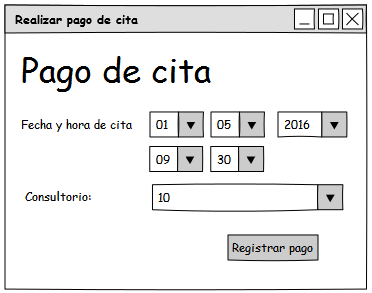
\includegraphics[width=0.8\textwidth]{images/IU_pagar_cita}
	\caption{IU Realizar pago de cita}
\end{figure}


\subsubsection{Salidas}
\begin{itemize} 
	\item Mensaje de confirmación: Cadena "Pago registrado correctamente"
	\item Información de cita:
	\begin{itemize}
		\item Fecha de cita: Fecha en formato dd/mm/yyyy
		\item Hora de cita: Hora con formato hh:mm
		\item Consultorio de cita: Número entero entre 1 y 12
	\end{itemize}
\end{itemize}
\subsubsection{Entradas}
\begin{itemize}
	\item ID de la cita: entero positivo
\end{itemize}

\subsubsection{Comandos}
\begin{itemize}
	\item \IUbutton{Registrar pago}:  Verifica que el la cita exista, tenga fecha y hora posterior a las actuales y haya sido pagada. En tal caso, se actualiza el estado de la cita a pagada.  \IUref{UI2}{Home}.	
\end{itemize}

\subsubsection{Mensajes}
\begin{Citemize}
	\item {\bf MSGa} Cita no existe
	\item {\bf MSGb} La cita expiró
	\item {\bf MSGc} Cita ya está pagada
\end{Citemize}

